\documentclass{article}

\usepackage{../arxiv}

\usepackage[utf8]{inputenc} % allow utf-8 input
\usepackage[T1]{fontenc}    % use 8-bit T1 fonts
\usepackage{hyperref}       % hyperlinks
\usepackage{url}            % simple URL typesetting
\usepackage{booktabs}       % professional-quality tables
\usepackage{amsfonts}       % blackboard math symbols
\usepackage{nicefrac}       % compact symbols for 1/2, etc.
\usepackage{microtype}      % microtypography
\usepackage{cleveref}       % smart cross-referencing
\usepackage{graphicx}
\usepackage{caption}
\usepackage{algorithm}
\usepackage{algpseudocode}
\usepackage{ragged2e}
\usepackage[style=numeric,sorting=none]{biblatex}
\usepackage[symbol]{footmisc}
\usepackage{tabu}
\usepackage{color}
\usepackage{nicefrac}

\addbibresource{\jobname.bib}

\title{Dango DEX}

\author{
  Larry Engineer \\
	Left Curve Software \\
	\texttt{larry@leftcurve.io} \\
}

\date{Initial version: UNRELEASED}

\begin{document}
\maketitle

\begin{abstract}
  Dango DEX is an onchain limit order book exchange that tackles three main challenges faced by today's DEXs: the inaccessibility of order book market making to retail investors due to the high level of sophistication required; reduced yield for AMM LPs due to arbitrage flow; and malicious MEV. Dango DEX enshrines its order book with a passive liquidity pool that actively adjusts its quotes utilizing a low latency oracle, and clears orders using frequent, uniform price, sealed bid auctions. Overall, Dango DEX seeks to democratize market making on order books, minimize toxic arbitrage flow, while maximize organic, non-arbitrage flow.
\end{abstract}

Dango DEX is one of the two flagship apps of our upcoming DeFi ecosystem, Dango,\supercite{dangotwitter} besides the cross-collateralized \textbf{credit account}. To learn more about the credit account, see \cite{creditaccountmarsforum,creditaccountbuidlkeynote}.

This paper is laid out as follows: 1) identifying the problems in today's DeFi exchanges; 2) analyzing the causes of the problems; and 3) proposing our solutions.

\section{Background}

\subsection{TradFi}

In traditional finance (TradFi) markets, \textbf{limit order book} (LOB) is the primary venue for trading. A limit order consists of the quantity of asset the trader wishes to buy or sell, and a limit price at which or better the trade must be executed.

\textbf{Market makers} (MMs) facilitate trades by strategically placing orders below and above the prevailing market price. E.g., suppose Apple stock (AAPL) is trading at \$200. An MM may place a \texttt{BUY} order at \$199.5 and a \texttt{SELL} order at \$200.5. The \$1 difference is known as the \textbf{spread}. If a trader sells AAPL to the MM by taking the said \texttt{BUY} order, then another trader buys AAPL by taking the said \texttt{SELL} order, the MM has made \$1. This is typically described as the MM ``making money on the spread''.

MMs bet the stock's price goes side ways, i.e. there is roughly the same buy and sell volume. If the market only goes one way, the MM accumulates one side of the inventory, which is the underperforming side. E.g., if there is consistently more sellers of AAPL than buyers, the MM's \texttt{BUY} orders get consistently picked up more often than his \texttt{SELL} orders do, he would accumuate a large inventory of AAPL, an asset that's going down in price. He would underperform the trading strategy that simply holds the initial inventory without market making. This is known as the \textbf{inventory risk} which is rooted in the asset's price volatility. MMs usually use \textbf{hedging} to mitigate this risk.

Another major risk faced by MMs comes from \textbf{information asymmetry}. Suppose Apple releases a better-than-expected earnings report, causing the ``fair value'' of its stock to jump to \$300. However, the MM is still placing orders around the \textbf{stale price} of \$200, either because he isn't aware of the news or is slow to update the quotes. An \textbf{informed trader} or \textbf{high frequency trader} (HFT) is one who is well informed on the news and is able to execute trades faster. The NFT is able to pick up the MM's \texttt{SELL} order at \$200.5 and immediately resell the stock for \$300, pocketing the arbitrage gain. The MM loses value because he has sold the stock at a much lower-than-market price. Both MMs and HFTs invest significant amount of resources to improve their execution speed in an ``arms race''.\supercite{frequentbatchauctions} This is a very high level of sophistication that makes market making inaccessible to most retail investors.

\subsection{DeFi}

Maintaining a LOB and executing orders is computationally costly. For this reason, onchain finance has historically relied on \textbf{constant function market makers} (CFMMs) instead of LOBs. (That is, until the recent advent of high performance blockchains such as Solana, Diem, Dydx, and Hyperliquid.)

A CFMM, instead of maintaining a book of limit orders, maintains a pool of liquidity and quotes prices based on a predefined \textbf{invariant}. An invariant is a function $f(x, y)$ that yields the same value before and after a trade, where $x$ and $y$ are the quantities of the \textbf{base asset} and the \textbf{quote asset}, respectively (known as the pool's \textbf{reserves}):

\begin{equation}
  f(x, y) = \mathrm{constant}
\end{equation}

Suppose a pool contains base asset $\mathtt{A}$ and quote asset $\mathtt{B}$ of reserves $A$ and $B$, respectively, and a trader wishes to swap $a$ amount of $\mathtt{A}$ into $\mathtt{B}$. The pool would determine the output amount $b$ by solving the equation:

\begin{equation}
  f(A, B) = f(A + a, B - b)
\end{equation}

Similarly, a swap from $b$ amount of $\mathtt{B}$ into $\mathtt{A}$ will have its output amount $a$ determined by:

\begin{equation}
  f(A, B) = f(A - a, B + b)
\end{equation}

Note that this doesn't consider trading fees. Since there is no such thing as ``spread'' in CFMMs as in LOBs, the pool makes money for its \textbf{liquidity providers} (LPs) by charging a fee on each trade. Specifically, a small portion of the trade's output is deducted and injected into the pool. The value of $K$ slightly increases as a result. As such, $K$ can be considered as a measurement of how much liquidity there is in the pool, regardless of the asset prices.

CFMMs share the same types of risks as LOBs, but to different degrees. Firstly, LPs in an CFMM pool bet the two assets' relative price stays roughly constant. If one asset's price drops relative to the other, the pool accumulates this underperforming asset. Not considering fees, this would underperform the strategy of simply holding the two assets and not market making. This is known as \textbf{impermanent loss} (IL). IL is essentially the same thing as inventory risk for LOBs, caused by the asset's volatility, and can be mitigated through hedging.

In terms of information asymmetry, however,  CFMMs are categorically worse than LOBs. A traditional CFMM \textit{never} adjusts its quotes in response to new information. Therefore, from an LP's perspective, a CFMM always trades at worse-than-market prices. The loss incurred from this is known as \textbf{loss-versus-rebalancing} (LVR).\supercite{lvr}

A \textbf{searcher} is a trader who scans onchain DEXs for stale prices, and executes CEX-DEX arbitrage. Since arbitraging is highly competitive, searchers share portions of their arbitrage gains with the chain's block builders by paying ``tips''.

There are other ways besides arbitrage with which searchers make money. Once of these is \textbf{sandwich attacks}, where a searcher bribes the block builders to insert transactions (txns) immediately before and after a user's trade. These txns manipulate prices in the DEX, give the user a worse execution price, while profiting the trader. Sandwich attack is not inheritly a problem of CFMMs; onchain LOBs can be similarly attacked. Instead, it's a result of the fact that user orders are broadcasted transparently through the network. In comparison, user orders in CEXs are kept private unless filled.

\subsection{The problems}

Through the above discussions, we have identified three problems with TradFi and DeFi exchanges:

\begin{enumerate}
  \item Market making in LOBs is not accessible to retail investors because of the high level of sophistication required, which is in larger part a result of the HFT arms race.
  \item CFMM democratizes market making to retail investors, but they generally don't make money or even lose money because of LVR.
  \item Traders are susceptible to sandwich attacks due to the lack of privacy.
\end{enumerate}

We do not aim to solve IL / inventory risk, because it's rooted in the assets' volalitity, not a problem with DEX design. We can imagine vaults that automatically deploy hedging strategies to mitigate it.

\section{Our solution}

We propose solving the above problems as follows:

\begin{itemize}
  \item Create a LOB that has an enshrined passive liquidity pool. The pool will place orders in the LOB following a CFMM invariant.
  \item In order to mitigate LVR, we:
        \begin{itemize}
          \item make available a high-frequency, low-latency oracle reporting the latest prevailing market prices;
          \item incorporate this oracle feed into the liquidity pool's CFMM invariant;
          \item give the pool priority in adjusting its quotes over other traders.
        \end{itemize}
  \item In order to mitigate MEV, we:
        \begin{itemize}
          \item use a private mempool so that user orders aren't public;
          \item use frequent, uniform price, sealed-bid auctions to match and execute orders, so that HFTs don't have time advantage over other traders.
        \end{itemize}
\end{itemize}

First, let's discuss how to incorporate a passive CFMM pool into a LOB.

\subsection{Passive liquidity on a LOB}

First, we introduce the concept of \textbf{marginal price}, $p_{\mathrm{m}}$. This is the price (defined as the units of quote asset that is equivalent in value as one unit of base asset) one gets if swapping an infinitesimal amount of base asset into the quote asset. It can be evaluated as:

\begin{equation}
  p_{\mathrm{m}} = - \frac{\mathrm{d}y}{\mathrm{d}x} = \frac{\frac{\partial f}{\partial x}}{\frac{\partial f}{\partial y}}
\end{equation}

Our passive liquidity pool will place \texttt{BUY} orders at prices below $p_{\mathrm{m}}$, \texttt{SELL} orders above $p_{\mathrm{m}}$, and no order at exactly $p_{\mathrm{m}}$.

Let us consider the \texttt{BUY} side first. Suppose the pool has reserves $A$ units of base asset and $B$ units of quote asset. Consider a swap that inputs $a$ units of base asset and outputs $b$ units of quote asset. The swap must follow the invariant:

\begin{equation}
  f(A, B) = f(A + a, B - b)
\end{equation}

We say this swap is executed at price $p = \frac{b}{a} < p_{\mathrm{m}}$.

We intrepret this as follows: the pool is willing to buy $a$ units of the base asset from counterparty traders at price $p$. In the context of LOB, this means the pool would put a cumulative \texttt{BUY} demand of quantity $a$ from $p_{\mathrm{m}}$ to $p$.

In reality, price is not continuous; the pool can only put orders at discrete \textbf{ticks}. Denote \textbf{tick size} as $\Delta p$, and the $n$-th tick below $p_{\mathrm{m}}$ as $p_n$:

\begin{equation}
  p_n = p_{\mathrm{m}} - n \Delta p \ \ (n = 0, 1, 2, \dots)
\end{equation}

If we find the pool places a cumulative \texttt{BUY} demand of quantity $a_n$ at price $p_n$, and quantity $a_{n-1}$ at price $p_{n-1}$, then obviously the order to be put at price $p_n$ is:

\begin{equation}
  \Delta a_n = a_n - a_{n-1}
\end{equation}

With $a_0 = 0$, we can iteratively work out $\Delta a_n$ for all $n = 1, 2, 3, \dots$; see \hyperref[alg:1]{Algorithm 1}.

\begin{algorithm}
  \caption{Determine \texttt{BUY} order sizes at ticks $p_n$, $n = 1, 2, 3, \dots$}
  \label{alg:1}
  \begin{algorithmic}
    \State $p_0 \gets p_{\mathrm{m}}$
    \State $a_0 \gets 0$
    \State $\Delta a_0 \gets 0$
    \For{n = 1, 2, 3, \dots}
    \State $p_n \gets p_{n-1} - \Delta t$
    \State $a_n \gets a: f(A, B) = f(A + a, b - p_n a)$ \Comment{Solve the invariant equation}
    \State $\Delta a_n \gets a_n - a_{n-1}$
    \EndFor
    \State \Return $[p_1, p_2, \dots]$, $[a_1, a_2, \dots]$, $[\Delta a_1, \Delta a_2, \dots]$
  \end{algorithmic}
\end{algorithm}

For the \texttt{SELL} side, the procedure is similar; \hyperref[alg:2]{Algorithm 2}.

\begin{algorithm}
  \caption{Determine \texttt{SELL} order sizes at ticks $p_n$, $n = 1, 2, 3, \dots$}
  \label{alg:2}
  \begin{algorithmic}
    \State $p_0 \gets p_{\mathrm{m}}$
    \State $a_0 \gets 0$
    \State $\Delta a_0 \gets 0$
    \For{n = 1, 2, 3, \dots}
    \State $p_n \gets p_{n-1} + \Delta t$
    \State $a_n \gets a: f(A, B) = f(A - a, b + p_n a)$ \Comment{Solve the invariant equation}
    \State $\Delta a_n \gets a_n + a_{n-1}$
    \EndFor
    \State \Return $[p_1, p_2, \dots]$, $[a_1, a_2, \dots]$, $[\Delta a_1, \Delta a_2, \dots]$
  \end{algorithmic}
\end{algorithm}

\subsection{Xyk}

The \textbf{xyk} invariant, proposed by Martin Köppelmann,\supercite{xykamm} has the form:

\begin{equation}
  f(x, y) = xy
\end{equation}

Marginal price can be found as:

\begin{equation}
  p_{\mathrm{m}} = \frac{y}{x}
\end{equation}

It's easy to solve that for the \texttt{BUY} side:

\begin{equation}
  a = -A + \frac{B}{p}
\end{equation}

For the \texttt{SELL} side:

\begin{equation}
  a = A - \frac{B}{p}
\end{equation}

\textbf{Example.} Consider a pool containing base asset SOL of quantity $A = 1$ and quote asset USD of quantity $B = 200$. marginal price $p_{\mathrm{m}} = 200$. Following \hyperref[alg:1]{Algorithms 1} and \hyperref[alg:2]{2} we can work out the order sizes in relation to tick price ($\Delta a_n$--$p_n$) and cumulative order depth ($a_n$--$p_n$), plotted in \hyperref[fig:1]{Figure 1}.

\begin{figure}
  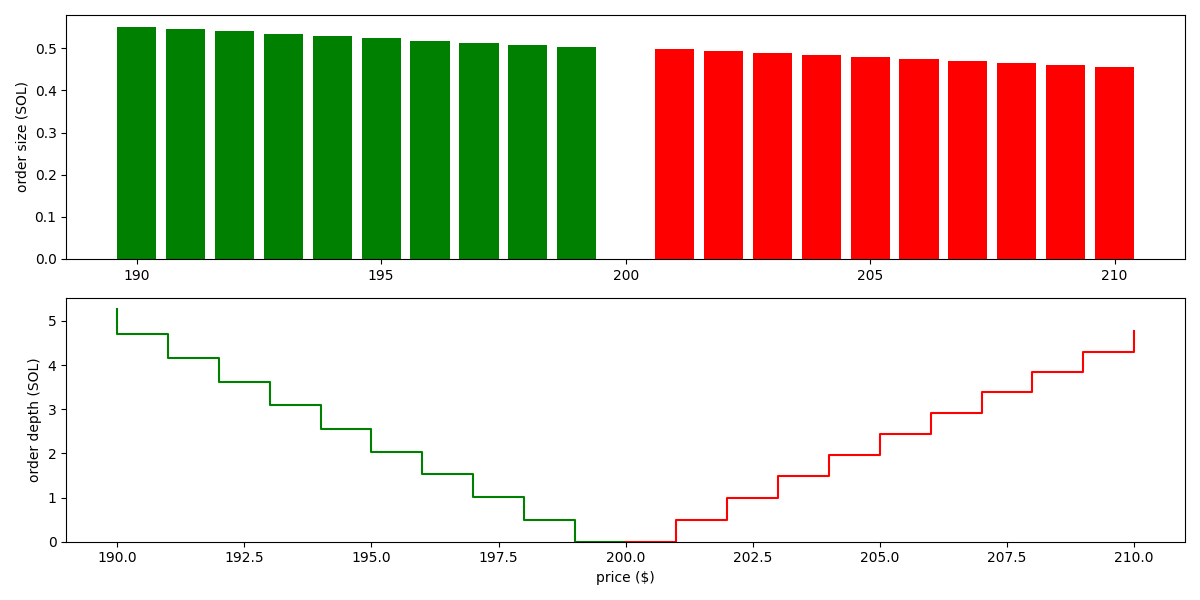
\includegraphics[width=\textwidth]{1-xyk.png}
  \caption{Order size and depth following the xyk invariant. $A = 1$, $B = 200$, $\Delta p = 0.1$.}
  \label{fig:1}
\end{figure}

We can see the pool puts liquidity roughly evenly over a wide range of prices. This capital inefficient; ideally, we want to concentrate the liquidity in the region close to $p_{\mathrm{m}}$.

Additionally, this invariant is susceptible to LVR, as $p_{\mathrm{m}}$ does not adjust in response to the change of price in CEXs.

\subsection{Solidly}

The Solidly invariant, conceived by Andre Cronje\supercite{andrecronjetwitter} and popularized by Velodrome and its forks,\supercite{velodrome,aerodrome} has the form:

\begin{equation}
  f(x, y) = x^3 y + x y^3 = K
\end{equation}

This formula assumes the two assets have the same price. In case they're not the same price, and we have an oracle feed indicating that one unit of $x$ is equivalent in value to $R$ units of $y$, the formula can be updated to:

\begin{equation}
  f(x, y) = x^3 \left( \frac{y}{R} \right) + x \left( \frac{y}{R} \right)^3
\end{equation}

The marginal price is:

\begin{equation}
  p_{\mathrm{m}}(x, y) = \frac{3 R^2 x^2 y + y^3}{R^2 x^3 + 3 x y^2}
\end{equation}

For convenience, let's denote:

\begin{equation}
  \alpha = A + a
\end{equation}

\begin{equation}
  \beta = \frac{B - p a}{R}
\end{equation}

Essentially, $\alpha$ is the pool's base asset reserve after the trade, $\beta$ is the quote asset reserve after the trade, adjusted for the oracle price.

The invariant equation:

\begin{equation}
  f(A, B) = f(A + a, B - p a) = \alpha^3 \beta + \alpha \beta^3
\end{equation}

This is a 4th-degree (quartic) equation, so finding a closed form solution is not feasible. Instead, we solve it using \textbf{Newton's method}. Define:

\begin{equation}
  g(a) = \alpha^3 \beta + \alpha \beta^3 - f(A, B)
\end{equation}

\begin{equation}
  g'(a) = -\frac{p}{R} \alpha^3 + a \alpha^2 \beta - \frac{3p}{R} \alpha \beta^2 + \beta^3
\end{equation}

We solve for $a$ such that $g(a) = 0$ following \hyperref[alg:3]{Algorithm 3}.

\begin{algorithm}
  \caption{Newton's method for solving $g(a) = 0$}
  \label{alg:3}
  \begin{algorithmic}
    \State $a_0 \gets A$
    \For{$i = 1, 2, 3, \dots$}
    \State $a_i \gets a_{i-1} - \frac{g(a_{i-1})}{g'(a_{i-1})}$
    \If{converge}
    \State \Return $a_i$ as the solution
    \EndIf
    \EndFor
  \end{algorithmic}
\end{algorithm}

The choice of the initial value $a_0$ is important. This is because $g(a) = 0$ has a trivial solution of $a = 0$, which corresponding to not placing an order at all. Instead, we want to find the non-trivial solution of $a > 0$. Emprically, choosing $a_0 = A$ always gives us the intended solution.

For the \texttt{SELL} side:

\begin{equation}
  \alpha = A - a
\end{equation}

\begin{equation}
  \beta = \frac{B + p a}{R}
\end{equation}

\begin{equation}
  g(a) = \alpha^3 \beta + \alpha \beta^3 - f(A, B)
\end{equation}

\begin{equation}
  g'(a) = \frac{p}{R} \alpha^3 - a \alpha^2 \beta + \frac{3p}{R} \alpha \beta^2 - \beta^3
\end{equation}

\textbf{Example.} Following the same example of SOL-USD pool in the previous discussions, assuming oracle price $R = 200$ (USD per SOL), the liquidity depth can be computed and plotted in \hyperref[fig:2]{Figure 2}. It's obvious that liquidity is now indeed concentrated around the marginal price.

\begin{figure}
  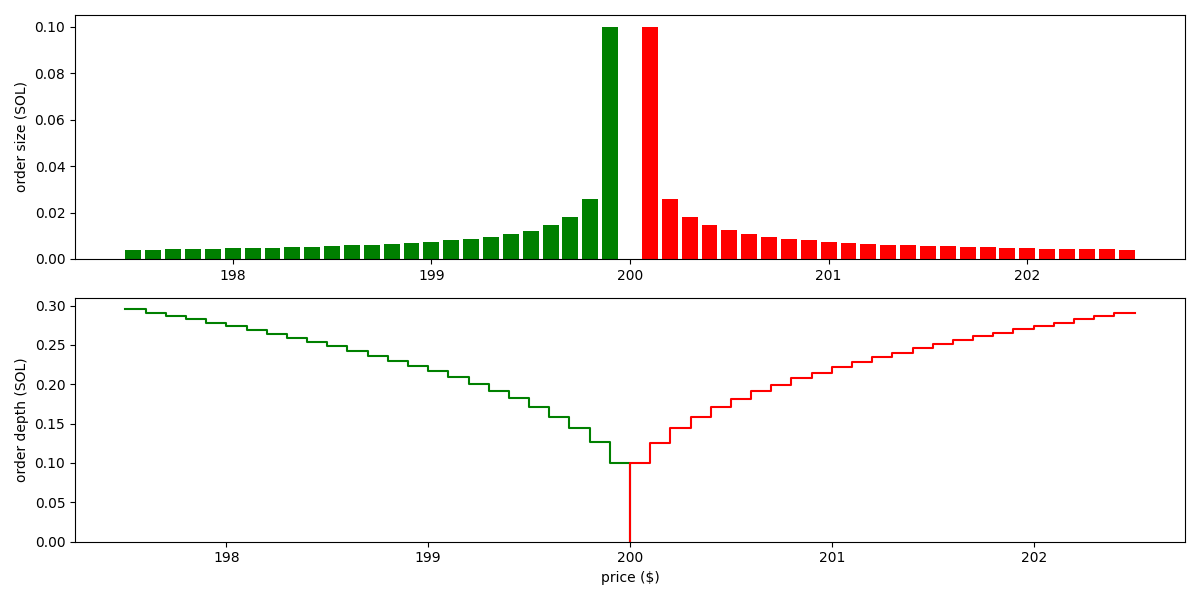
\includegraphics[width=\textwidth]{2-solidly.png}
  \caption{Order size and depth following the Solidly invariant. $A = 1$, $B = 200$, $\Delta p = 0.1$, $R = 200$.}
  \label{fig:2}
\end{figure}

In general, however, $R$ does not match exactly the composition of the pool reserves. In TradFi, MMs typically respond to this by adjusting the spread.\supercite{avellanedastoikov} Consider the situation where SOL appreciates to $R = 210$, a 5\% deviation from the pool's reserve composition of 1:200. In this case, a TradFi MM would \textit{increase} the bid spread and \textit{decrease} the ask spread. Thus, there is a higher probability the asks are picked up by noise traders, such that the MM offloads SOL and intakes USD, trending towards a rougly 1:1 ratio for value of the two assets.

How will our passive liquidity pool respond to this situation? Let's plot it in \hyperref[fig:3]{Figure 3}. As we see, the pool keeps the same spread on each side, but on the \texttt{SELL} side a bigger order size. This indicates the pool has a similar tendency of offloading SOL and intaking USD in this situation.

\begin{figure}
  \centering
  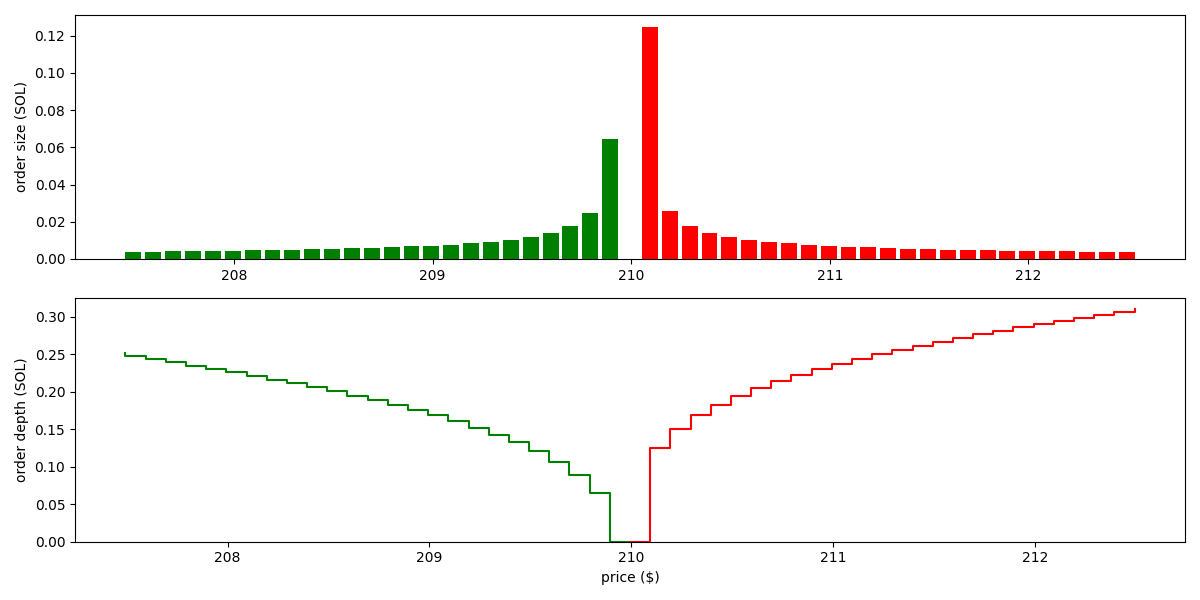
\includegraphics[width=\textwidth]{3-solidly-price-jump.png}
  \caption{Order size and depth following the Solidly invariant. $A = 1$, $B = 200$, $\Delta p = 0.1$, $R = 210$.}
  \label{fig:3}
\end{figure}

\subsection{Parameterization}

In the above formulation of the passive liquidity pool, the pool places orders every tick, starting one tick above and below $p_{\mathrm{m}}$. This can be customized by introducing two additional parameters:

\begin{itemize}
  \item \textbf{Cadence}: The pool can instead place an order every $N$ ticks. Alternatively, it can place orders more densely when close to $p_{\mathrm{m}}$, but more loosely when farther away. Either way, there will be fewer orders overall, reducing computational cost.
  \item \textbf{Spread}: The pool can place orders a few ticks further away from $p_{\mathrm{m}}$. A bigger spread may improve the pool's profitability. We may also consider adjusting the spreads in response to inventory inbalance.\supercite{avellanedastoikov}
\end{itemize}

\subsection{Minimizing LVR with oracle-imformed CFMM}

In order for the passive liquidity pool to provide accurate quotes, it's important that:

\begin{itemize}
  \item it has access to a low-latency oracle that accurately reports the up-to-date market prices; and,
  \item it must be able to adjust its orders before any other trader is able to pick up the stale quotes.
\end{itemize}

For the oracle, we propose using Pyth Laser,\supercite{pythlaser} which provides ultra fast price feeds with 1 millisecond updates. Each block, the proposer fetches the prices and submit them onchain in a transaction on the very top of the block.

To ensure the passive liquidity pool has priority in updating quotes, we utilize a technique which we dub \textbf{virtual order book}. Instead of physically placing orders, the pool constructs a virtual order book, based on its asset reserves and oracle price, prior to any order being matched. The matching engine then combines the real, physical order book with the virtual book before performing matching.

\subsection{Mitigating MEV with frequent batch auctions}

A searcher relies on two prerequisites both being satisfied in order to pull off malicious MEV activities:

\begin{itemize}
  \item user orders are broadcasted transparently, unencrypted, through the public p2p network;
  \item trades are possibly executed at different prices throughout the same block.
\end{itemize}

On the first point, we believe the endgame solution is implementing an encrypted mempool.\supercite{encryptedmempool} We may do this, however, to achieve a faster go-to-market, we propose an interim solution: 1) the Dango chain to temporarily run on a proof-of-authority validator set; 2) validators to configure their mempools such that they only receive transactions, and broadcast only to other validators, but not to any other node; 3) users to broadcast their transactions directly to the validators. As such, one can assume validators themselves do not engage in malicious MEV, and user transactions can be considered private.

On the second point, we propose to execute orders using the frequent batch auctions (FBAs) approach.\supercite{frequentbatchauctions,frequentbatchauctions2} Specifically, the flow of a block would be:

\begin{enumerate}
  \item In the first transaction, the proposer submits up-to-date oracle prices.
  \item Users submit orders. These orders are stored in a \textbf{transient storage} in the DEX smart contract. Data in the transient storage only persists through one block (wiped at the end of the block) and importantly, cannot be queried by other contracts.
  \item After all user transactions have been processed, the DEX contract iterates through all trading pairs that have received new orders in this block and attempts to match the orders:
        \begin{enumerate}
          \item Add new orders in the transient storage into the order book.
          \item Compute the virtual order book of the passive liquidity pool, based on the pool's asset reserves and oracle price.
          \item Combine the two books in (a) and (b) and perform order matching through a uniform price auction.\supercite{uniformpriceauctions} The objective is to find the intersection between the cumulative supply and demand curves, which is the price that maximizes trading volume.
          \item Given the clearing price found in (c), fill the orders, send the output funds to traders.
        \end{enumerate}
\end{enumerate}

There are two notable elements in this:

\begin{itemize}
  \item This is a \textbf{sealed-bid} auction. Given that users broadcast transactions to a private mempool, and orders are stored in the transient storage, the orders are kept confidential prior to the auction.
  \item This is a \textbf{uniform price} auction. All trades are settled at the same clearing price, so it's literally impossible to execute sandwich attacks.
\end{itemize}

\section{Conclusion}

We have identified, analyzed the causes of, and proposed Dango DEX as a solution to three main problems of today's decentralized exchanges:

\vskip 2.6px
\tabulinesep=2mm
\newcolumntype{Y}{>{\RaggedRight}X[m]} % avoid hyphenation when wrapping words in tabularx
\begin{tabu} to \textwidth {YYY}
  \toprule
  \textbf{The problem}                                                                                       & \textbf{The cause} & \textbf{Our solution} \\
  \midrule
  Market making on LOBs is not accessible for retail investors                                               &
  High level of sophistication is required                                                                   &
  Our LOB to be enshrined with a passive liquidity pool that follows the Solidly AMM curve                                                                \\
  \hline
  LVR                                                                                                        &
  CFMMs do not actively adjust quotes in reaction to changes in asset prices                                 &
  Our passive liquidity pool to adjust its curve based on a low-latency oracle feed, with priority over any other trader                                  \\
  \hline
  MEV                                                                                                        &
  User orders are broadcasted publicly, and are settled at potentially different prices throughout the block &
  Private mempool; frequent sealed-bid batch auctions at uniform prices                                                                                   \\
  \bottomrule
\end{tabu}

\printbibliography

\end{document}
